
\subsection{katz-eig}

\textit{Compare different optimization approaches w.r.t. runtime and evaluation metric}

The strategies for optimizing algorithm parameters for different datasets, or parameter tuning, has focused on keeping $\beta$ fixed and searching for $K$ which optimizes \textit{F-measure}. The analysis in \sectionref{sec:param:katzeig} showed that varying $\beta$ has a small effect on the algorithm's performance. So $\beta$ was fixed to $\beta = \frac{1}{\|A_{train}\|_2}$.

What follows is a description of the different optimization techniques evaluated:

\begin{description}
    \item[grid]
        Does a grid search over $K$, with a fixed step size. $\beta$ was fixed. $0 < K \leq 50$ was examined and a step size of 1 was used.
    \item[rand]
        A random sampling over a subspace of $K$ with a fixed $\beta$. Depends on the size of the subset to sample over and the number of samples. $0 < K \leq 50$ was examined and 12 random samples were used meaning 24\% of the subspace was examined.
    \item[hill]
        Simple hill climbing algorithm which examines the neighbours of $K$. Uses a fixed $\beta$. Will find a local optima. A step size of 1 was used.
    \item[stoch-hill]
        An extension of the hill climbing algorithm which does a random restarts whenever a local optima is found. Also randomly jumps to a random $K$. Depends on the random jump probability, the subspace of $K$ and the number of iterationss. A step size of 1 was used and the restrinction was $0 < K \leq 50$. 12 samples were used meaning 24\% of the subspace was examined.
\end{description}

\begin{figure}[h!]
    \centering
    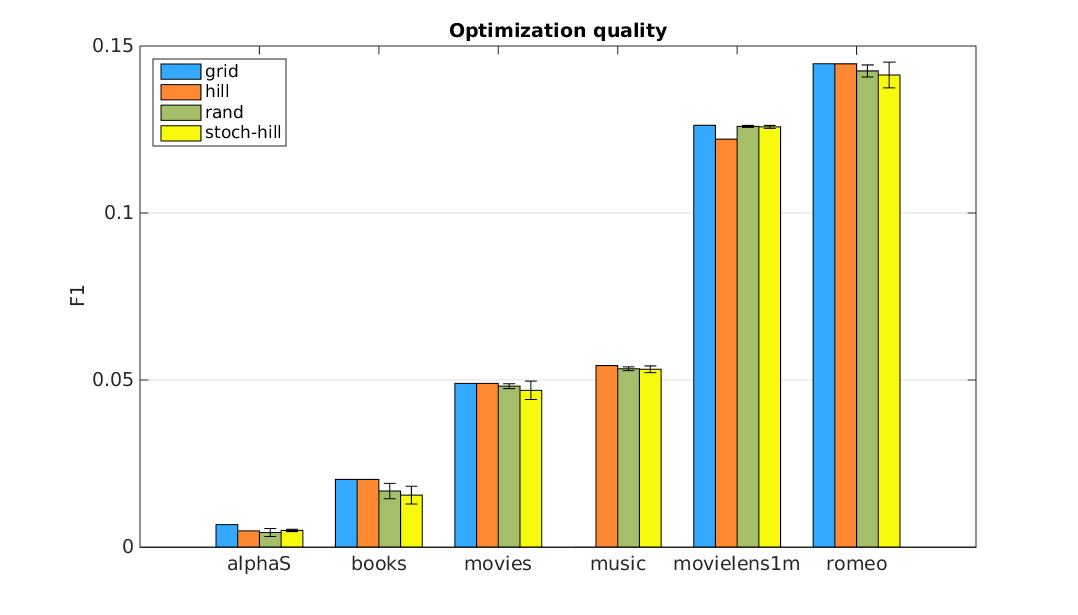
\includegraphics[width=0.9\textwidth]{fig/comp/comp_katz_quality.png}
    \caption{Comparison of the recommendation quality given from the parameters found by thedifferent optimization strategies for \textit{katz-eig}.}
\end{figure}

\begin{figure}[h!]
    \centering
    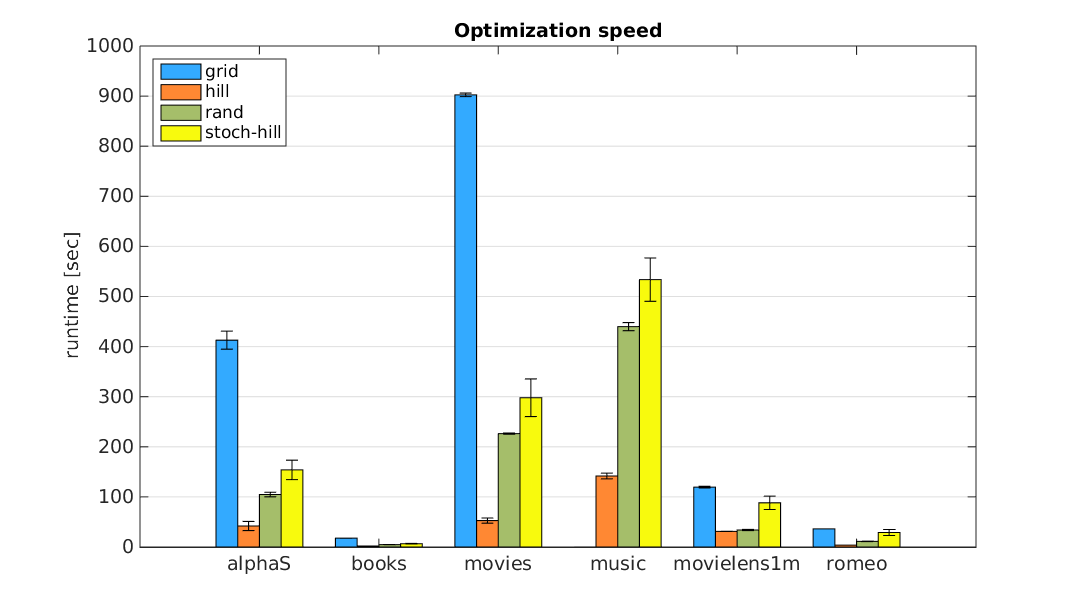
\includegraphics[width=0.9\textwidth]{fig/comp/comp_katz_speed.png}
    \caption{Comparison of the runtime of the different optimization strategies for \textit{katz-eig}, given the optimized parameters specified in \appendixref{app:opt_params}.}
\end{figure}

\begin{figure}[h!]
    \centering
    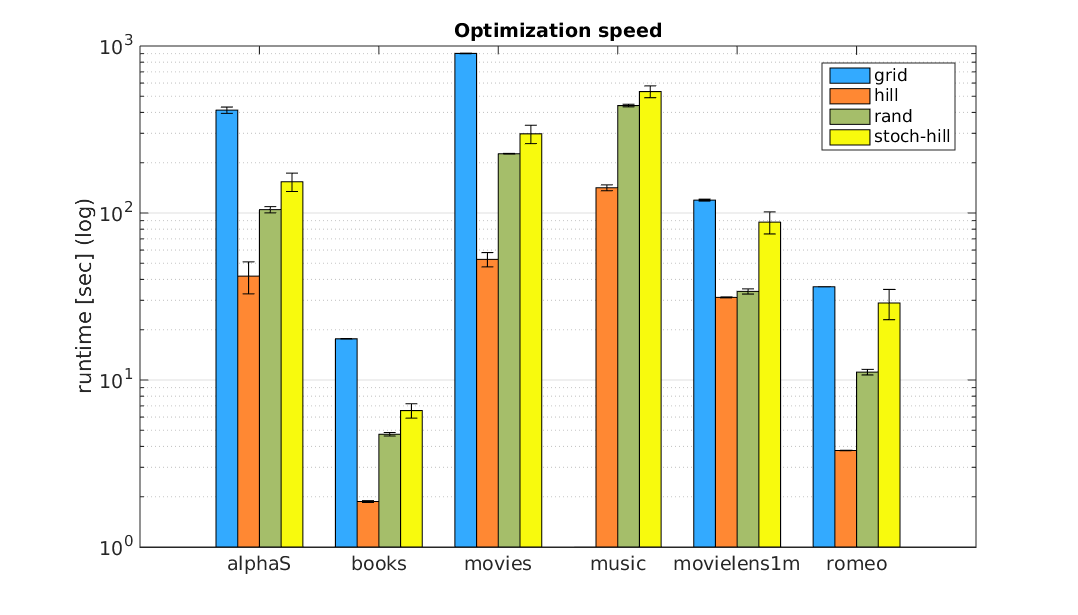
\includegraphics[width=0.9\textwidth]{fig/comp/comp_katz_speed_log.png}
    \caption{Comparison of the runtime of the different optimization strategies for \textit{katz-eig}, given the optimized parameters specified in \appendixref{app:opt_params}. In a log scale.}
\end{figure}

\FloatBarrier
